\section{Free-form generation: a matched-prefix test of mid-sequence repair}
\label{sec:sequential}

Correction looks more attractive in captions than in yes/no answers: replacing a hallucinated word keeps a
caption that deletion would damage. The extension seems mechanical, and two obstacles are known. Editing a prefix makes
later tokens off-policy, which is feedback covariate shift \citep{fannjiang2022fcs} and falls outside weighted conformal
methods \citep{tibshirani2019}; and per-claim guarantees say nothing about a whole sequence whose length is
data-dependent. Prefix-conditional (Mondrian) $p$-values and e-processes \citep{waudbysmith2024,ramdas2023} could
handle both in principle, leaving the drift of the calibration pool, which on-policy calibration by fixed-point
iteration would address if the correction map were monotone. We measured whether it is before attempting a proof.

\paragraph{Design}
For each image we generate a caption greedily, locate the first hallucinated object mention at position $t$ using AMBER's
per-image present and absent object lists, and build two prefixes identical up to $t$: one that keeps the hallucinated
word and one that substitutes the best-detected object the image contains. We continue decoding the same number of
tokens from each and count hallucinated mentions in the continuations only. The only difference between the two
continuations is the intervention. The unit is the matched pair ($n=121$ images); there is one repair per pair.

\paragraph{Result}
In this sample repair makes the continuation worse (Table~\ref{tab:monotone}, Figure~\ref{fig:monotonicity}). Hallucinated mentions
in the continuation rise from $1.207$ to $1.413$, a paired difference of $+0.207\pm0.091$ ($t(120)=2.27$, two-sided
$p=0.025$), with $45$ pairs worsening, $25$ improving and $51$ tied. A Wilcoxon signed-rank test ($p=0.035$) and an exact sign test
($p=0.023$) agree. The Hodges--Lehmann estimate is $0.000$ because $42\%$ of pairs are tied.

\begin{table}[t]
\centering
\caption{Paired matched-prefix test ($n=121$). All $p$-values are two-sided.}
\label{tab:monotone}
\small
\begin{tabular}{lccc}
\toprule
Downstream measure (continuation only) & Original & Repaired & paired difference ($p$)\\
\midrule
Hallucinated mentions (mean)      & 1.207 & 1.413 & $+0.207$ ($0.025$)\\
Hallucinations per $100$ words    & 3.61  & 4.30  & $+0.75$ ($0.011$)\\
Faithful mentions (mean)          & 1.579 & 1.752 & $+0.174$ ($0.077$)\\
Continuation length (words)       & 33.4  & 32.9  & $-0.55$ ($0.092$)\\
Hallucinated share of mentions    & 0.433 & 0.447 & $-0.004$ ($0.884$)\\
\bottomrule
\end{tabular}
\end{table}

\begin{figure}[t]
\centering
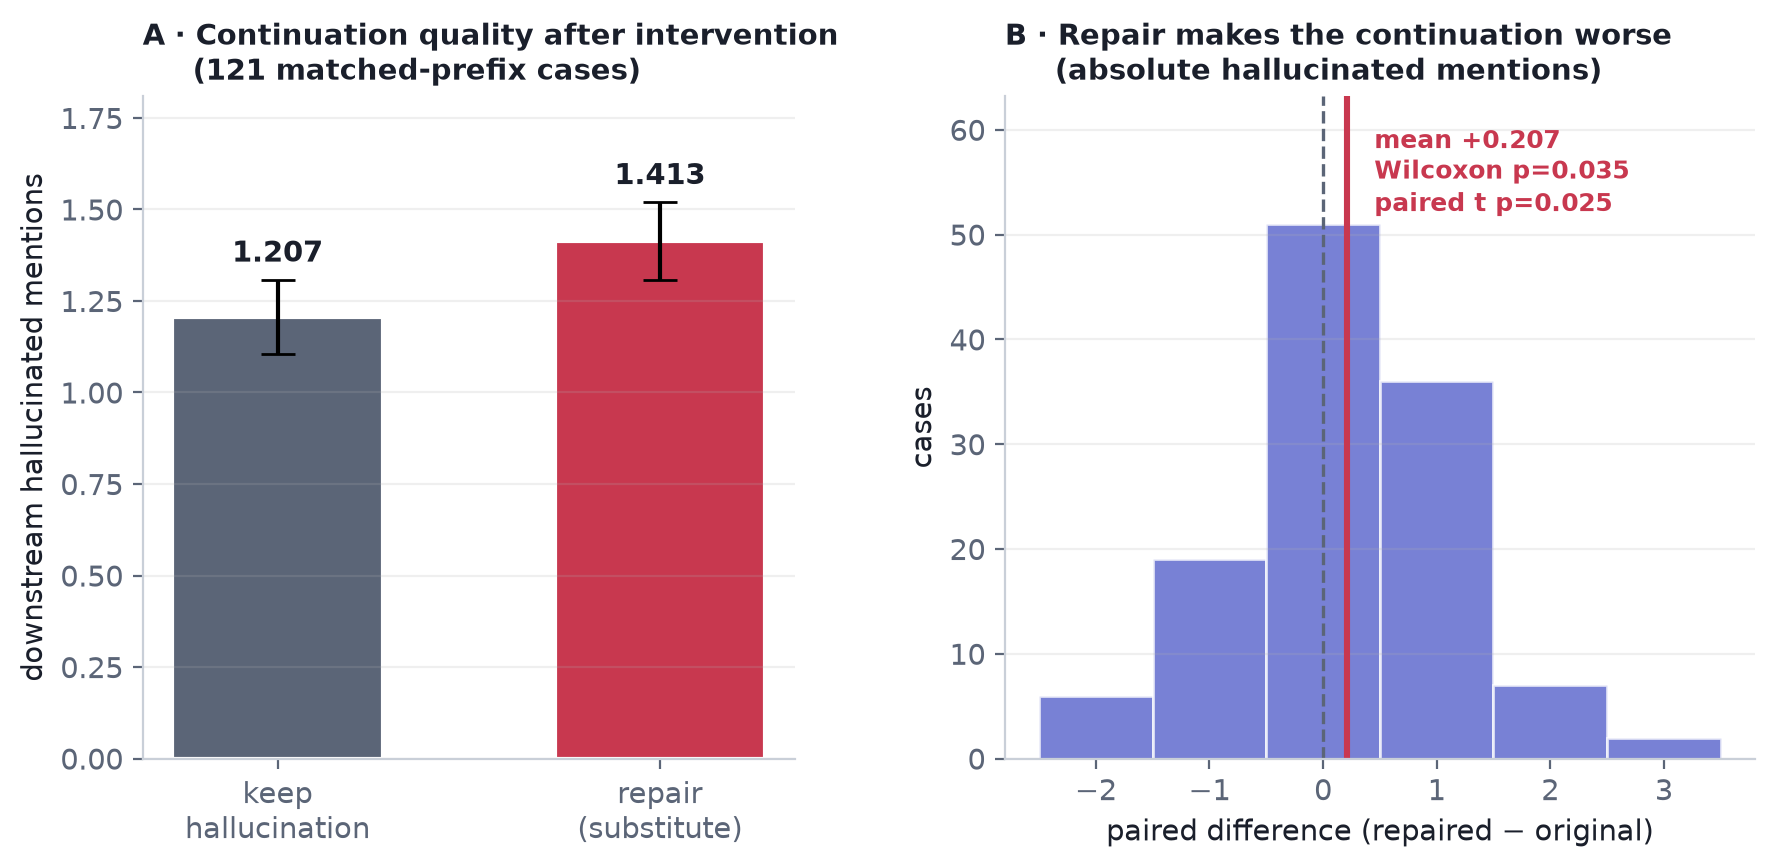
\includegraphics[width=0.9\textwidth]{fig_monotonicity.png}
\caption{(A) Mean hallucinated mentions in the continuation after keeping or repairing the flagged claim (standard errors).
(B) Distribution of the paired difference.}
\label{fig:monotonicity}
\end{figure}

\paragraph{What the experiment can support}
The result is significant under three tests and under-powered. At the observed paired standard deviation ($0.999$) the
minimum detectable effect at $80\%$ power is $+0.257$, larger than the observed $+0.207$, and about $186$ pairs would be
needed at this effect size. Equivalence testing against a margin of $\pm0.25$ does not establish equivalence
($p=0.317$). The sign is established and the magnitude is not: any value in $[+0.027,+0.386]$ is compatible. The number
of hallucinated mentions rises together with faithful mentions and with mention density; per mention, the hallucinated share does not move
($0.433\to0.447$, $p=0.884$), so the mechanism is denser object talk after repair. A certificate on the count of false
claims is not helped by this, since each additional hallucinated mention counts. The substitution used here is
context-blind, and the finding concerns that rule rather than all correction. What the data withdraw is support
for a monotone correction map and hence for a fixed-point route to a sequential guarantee, at the sample size we have.

\paragraph{A coupling bound}
For a sequence of claims let $F(O)$ be the number of false claims and $\Risk(O)=\E[F(O)]$ the expected count per
sequence. Let a repair rule replace claims at a random set $P$ of positions, producing $O'$.
Write $W$ for the number of wrong repaired claims, $F_P(O)$ for the number of false \emph{original} claims at the
repaired positions, and $\Delta$ for the signed change in the number of false claims at non-repaired positions
between $O'$ and $O$.

\begin{theorem}[Coupling bound for corrected sequences]
\label{thm:coupling}
$F(O')=F(O)-F_P(O)+W+\Delta$ pointwise, hence
\[
\Risk(O')=\Risk(O)+\E[W]-\E[F_P(O)]+\Iota\ \le\ \Risk(O)+\E[W]+\Iota,\qquad \Iota:=\E[\Delta].
\]
$\Iota$ is signed: a repair that prevents later errors makes it negative. If at most one claim is repaired per
sequence, $\E[W]=\Pr[X\in R]\,\Pr[\text{repair wrong}\mid X\in R]$; in general $\E[W]=\sum_t\Pr[t\in P,\ \text{repair at }t\text{ wrong}]$ is an expected
count over repair opportunities.
\end{theorem}
\begin{proof}
The false claims of $O'$ are those at repaired positions (the wrong repairs, $W$) plus those at non-repaired positions. The false claims of $O$ are
those at repaired positions ($F_P(O)$) plus those at non-repaired positions. Subtracting gives the identity, and taking
expectations gives the equality; $F_P(O)\ge0$ gives the bound.
\end{proof}

In the matched-prefix experiment one claim is repaired per pair, so $\widehat\Iota$ is the paired difference in
the continuation: $+0.207\pm0.091$ additional false claims per repair. That is as large as the direct term for a
repair that is wrong with probability $0.2$, and it cannot be dropped. Certifying $\Risk(O)\le\alpha_1$ and the direct term by
$\alpha_2$ at $\delta/2$ each gives $\Risk(O')\le\alpha_1+\alpha_2+\Iota$ at $1-\delta$, which is useful only
relative to an already-selective base policy, since certifying the uncorrected generation is the object the
abstention floor makes expensive. A sequential procedure would have to price the continuation and not only the claim,
for example by searching over rewrites under an accumulated risk ledger. We leave that open.
